\documentclass[tikz,border=2pt]{standalone}
\usepackage{amsmath}
\usetikzlibrary{arrows.meta}
\begin{document}
% M/G/1 sample path: arrivals at 0, 0.6, 1.4, 3.8, 6.0, 6.5 (blue); services 2.0, 1.0, 1.5, 0.8, 1.2
% give departures at 2.0, 3.0, 4.5, 5.3, 7.2 (red). Left-behind numbers L_k = L(D_k) = 2, 1, 1, 0, 1 (green),
% consistent with L_k = [L_{k-1}-1]^+ + Y_k, Y = (2, 0, 1, 0, 1).
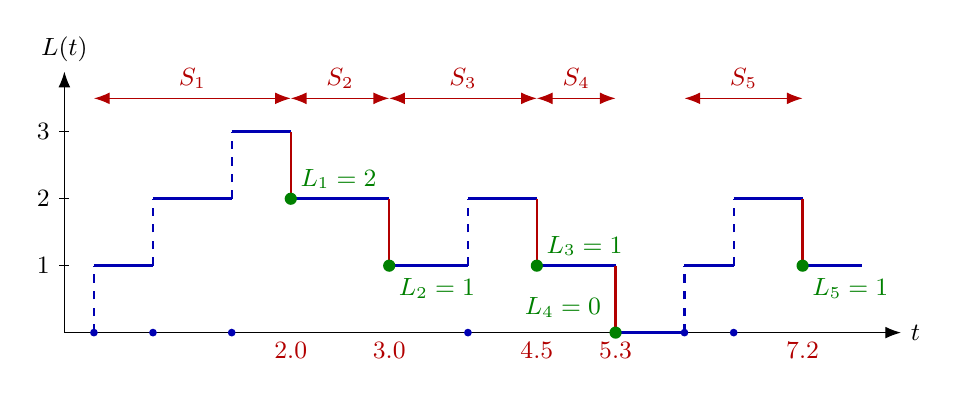
\begin{tikzpicture}[font=\small, >={Latex[length=2mm]}, x=1.25cm, y=0.85cm]
  \draw[->] (-0.3,0) -- (8.2,0) node[right] {$t$};
  \draw[->] (-0.3,0) -- (-0.3,3.9) node[above] {$L(t)$};
  \foreach \y in {1,2,3} \draw (-0.35,\y) -- (-0.25,\y) node[pos=0, left] {$\y$};
  % sample path
  \draw[blue!70!black, very thick]
    (0,1) -- (0.6,1) (0.6,2) -- (1.4,2) (1.4,3) -- (2.0,3) (2.0,2) -- (3.0,2) (3.0,1) -- (3.8,1)
    (3.8,2) -- (4.5,2) (4.5,1) -- (5.3,1) (5.3,0) -- (6.0,0) (6.0,1) -- (6.5,1) (6.5,2) -- (7.2,2) (7.2,1) -- (7.8,1);
  % arrival jumps
  \foreach \a/\lo in {0/0,0.6/1,1.4/2,3.8/1,6.0/0,6.5/1} {
    \draw[blue!70!black, thick, dashed] (\a,\lo) -- (\a,\lo+1);
    \fill[blue!70!black] (\a,0) circle (1.4pt);
  }
  % departures and left-behind values
  \foreach \d/\lk/\k in {2.0/2/1,3.0/1/2,4.5/1/3,5.3/0/4,7.2/1/5} {
    \draw[red!70!black, thick] (\d,\lk+1) -- (\d,\lk);
    \fill[green!50!black] (\d,\lk) circle (2.2pt);
    \node[red!70!black, below] at (\d,0) {$\d$};
  }
  \node[green!50!black, anchor=south west] at (2.0,2.0) {$L_1=2$};
  \node[green!50!black, anchor=north west] at (3.0,0.95) {$L_2=1$};
  \node[green!50!black, anchor=south west] at (4.5,1.0) {$L_3=1$};
  \node[green!50!black, anchor=south east] at (5.25,0.08) {$L_4=0$};
  \node[green!50!black, anchor=north west] at (7.2,0.95) {$L_5=1$};
  % service intervals
  \foreach \s/\e/\lab in {0/2.0/S_1,2.0/3.0/S_2,3.0/4.5/S_3,4.5/5.3/S_4,6.0/7.2/S_5} {
    \draw[<->, red!70!black] (\s,3.5) -- (\e,3.5) node[midway, above] {$\lab$};
  }
\end{tikzpicture}
\end{document}
